%%=============================================================================
%% Methodologie
%%=============================================================================

\chapter{\IfLanguageName{dutch}{Methodologie}{Methodology}}%
\label{ch:methodologie}

\subsection*{Fase 1: Opstellen van de requirements}%
\label{sec:opstellen-van-de-requirements}
Om de onderzoeksvraag te beantwoorden is het belangrijk 
de requirements te analyseren. De opgestelde requirements zullen de basis vormen voor de beoordeling, de vergelijkende analyse en de proof of concept.
Deze vereisten zullen door diverse bronnen opgesteld worden. Als eerste
zullen de belangrijkste vereisten in de voorgaande literatuurstudie onderzocht worden. Vervolgens zal er een vraag
worden gesteld die mijn copromotor zal beantwoorden. De vraag bestaat uit: welke vereisten zijn volgens u belangrijk bij het kiezen van een 
LCNC platform en rangschik deze vereisten van belangrijk naar minder belangrijk. Op deze manier kan men een duidelijk beeld weergeven waarmee er rekening gehouden moet worden 
bij het evalueren van de Low-Code en/of No-Code platformen. De gekozen vereisten kan men terugvinden in Hoofdstuk~\ref{ch:vereisten}.

\subsection*{Fase 2: Analyse van de alternatieven}%
\label{sec:analyse-van-de-alternatieven}
In deze fase zal er een onderzoek uitgevoerd worden naar alternatieve platformen.
Hierbij zal er een online onderzoek gebeuren waarbij men bronnen zal gebruiken zoals 
officiële websites, reviews en technologieblogs. Vervolgens zal er per platform de 
voordelen, nadelen en beschrijvende informatie worden opgenomen. Daarna komen 
de belangrijkste eigenschappen van een platform terecht in een tabel waarbij de criteria
van de requirements analyse zullen worden opgenomen. Hieruit volgt een selectie van een 
alternatief die verder zal worden geanalyseerd. Deze fase kan men terugvinden in Hoofdstuk~\ref{ch:evaluatie-en-selectie-van-alternatieven}.


\subsection*{Fase 3: Vergelijkende analyse}%
\label{sec:vergelijkende-analyse}
In deze fase vergelijken we Softr, Stacker en Bubble met elkaar.
Hieruit volgt dat men per criterium bekijkt welke van de drie het beste scoort. Dit zal gebeuren door middel van verschillende bronnen.
In de volgende fase zal er een Proof of Concept uitgevoerd worden om de gebruiksvriendelijkheid en andere criteria zoals platformflexibiliteit te testen.
De vergelijkende analyse is terug te vinden in Hoofdstuk~\ref{ch:vergelijkende-analyse}.

\subsection*{Fase 4: Proof of Concept}%
\label{sec:proof-of-concept}
Om de gebruiksvriendelijkheid en andere criteria's zoals platformflexibiliteit en snelheid van het platform te testen, is er een Proof of Concept uitgevoerd. 
\\
\\
Een deel van de Proof-Of-Concept is uitgevoerd door drie niet-programmeurs die geen IT achtergrond hebben. De testpersonen moeten
een kleine applicatie maken met twee verschillende platformen. De applicatie is een eenvoudige task app waarbij je taken kan toevoegen en kan bekijken.
\\
\\
Het zal dus bestaan uit een home scherm waar je alle taken ziet en een scherm om een nieuwe taak toe te voegen. De task app zal met hulp van de organisator geconnecteerd worden met een gegevensopslagplatform zoals Airtable of Google Spreadsheets, indien nodig. 
Vervolgens zal MAKE.com niet geïntegreerd worden in de applicatie omdat dit te verwarrend en moeilijk is voor niet-programmeurs zonder IT-ervaring.
De niet-programmeurs mogen ook hulp vragen via het internet en aan de organisator.
Elke niet-programmeur zal slechts twee van de drie platformen testen in een verschillende volgorde, waardoor elk platform 2 keer zal getest worden. Dit maakt efficiënter gebruik van hun tijd en middelen waardoor de platformen grondiger geëvalueerd kunnen worden. De volgorde van het testen zorgt voor het verminderen van leereffecten, wat leidt tot eerlijkere en objectievere evaluaties.
Hieronder bevindt zich ook een ontwerp van de applicatie als leidraad.
\\
\begin{figure}[H]
    \centering
    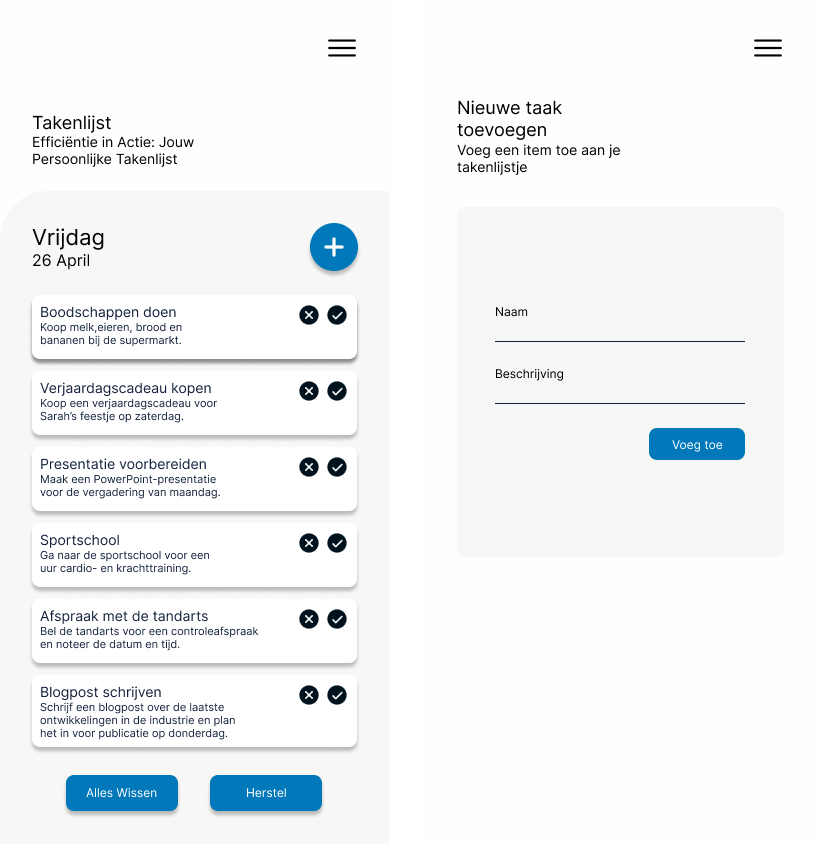
\includegraphics[scale=0.4]{todo_app_poc.png}
    \caption[Voorbeeld van een mogelijke TODO app]{Voorbeeld van een mogelijke TODO app\\\textcopyright\ Joeri Verhelst}
    \label{fig:todo_app}
\end{figure}

Daarnaast zal een programmeur een andere app maken, genaamd een feedback app, die bestaat uit een formulier voor feedback dat data opslaat in AirTable.
Vervolgens zal ook via MAKE.com een e-mail gestuurd worden naar de gebruiker die feedback heeft gegeven.
Dit zorgt ervoor dat men de integratie met zowel AirTable als MAKE.com kan testen. Daarnaast zal de applicatie ook een lijst bevatten van alle feedback.
Hieronder bevindt zich ook een ontwerp van de applicatie als leidraad.

\begin{figure}[H]
    \centering
    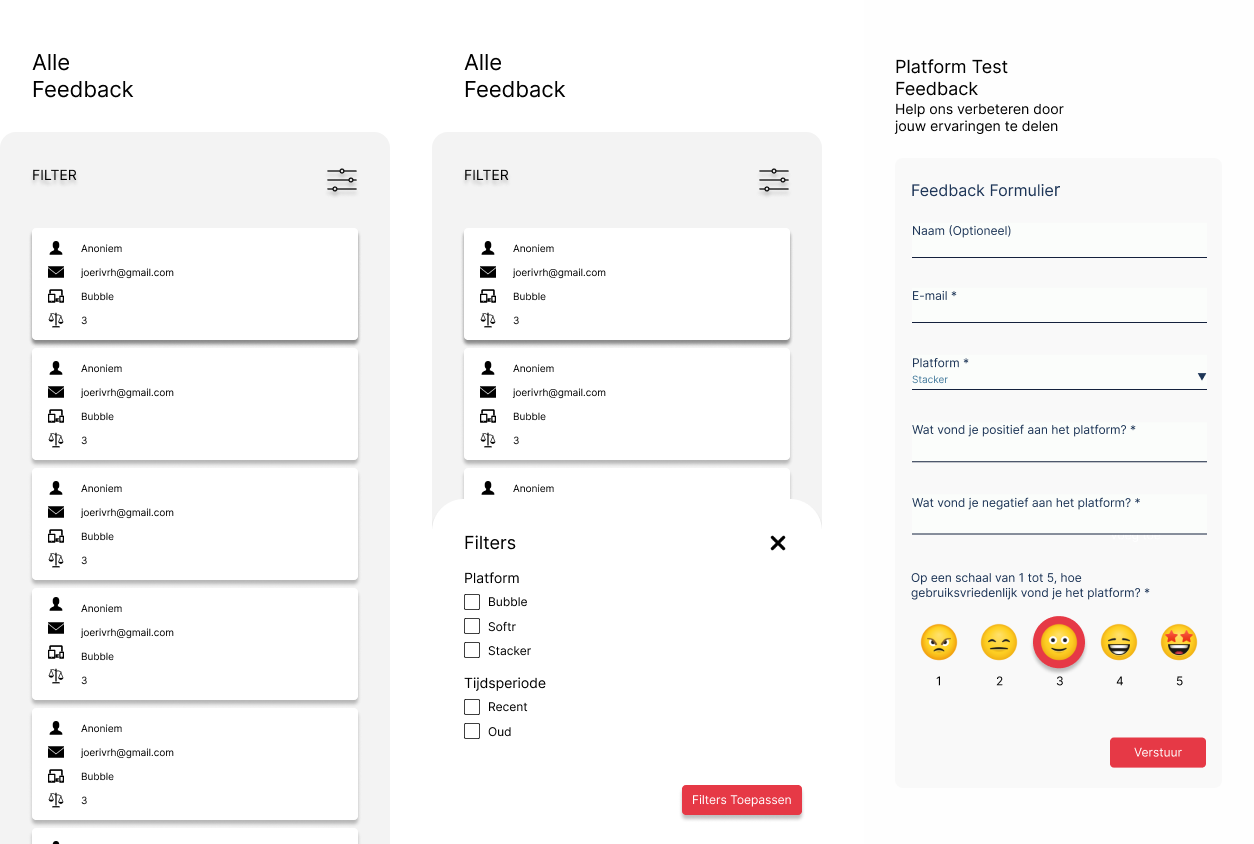
\includegraphics[scale=0.35]{feedback_app_poc.png}
    \caption[Voorbeeld van een mogelijke feedback app]{Voorbeeld van een mogelijke feedback app\\\textcopyright\ Joeri Verhelst}
    \label{fig:feedback_app}
\end{figure}
Het is \textbf{belangrijk} om te vermelden. Dit door het beperkte aantal testpersonen en het gebrek aan tijd om elk platform uitgebreid te evalueren dat 
de uitgevoerde proof of concept niet voldoende is om een definitieve beslissing te nemen over welk platform het beste is voor Quivvy Solutions.
\\
\\
U kunt de uitgevoerde Proof of Concept terugvinden in Hoofdstuk~\ref{ch:proof-of-concept}.

%% TODO: In dit hoofstuk geef je een korte toelichting over hoe je te werk bent
%% gegaan. Verdeel je onderzoek in grote fasen, en licht in elke fase toe wat
%% de doelstelling was, welke deliverables daar uit gekomen zijn, en welke
%% onderzoeksmethoden je daarbij toegepast hebt. Verantwoord waarom je
%% op deze manier te werk gegaan bent.
%% 
%% Voorbeelden van zulke fasen zijn: literatuurstudie, opstellen van een
%% requirements-analyse, opstellen long-list (bij vergelijkende studie),
%% selectie van geschikte tools (bij vergelijkende studie, "short-list"),
%% opzetten testopstelling/PoC, uitvoeren testen en verzamelen
%% van resultaten, analyse van resultaten, ...
%%
%% !!!!! LET OP !!!!!
%%
%% Het is uitdrukkelijk NIET de bedoeling dat je het grootste deel van de corpus
%% van je bachelorproef in dit hoofstuk verwerkt! Dit hoofdstuk is eerder een
%% kort overzicht van je plan van aanpak.
%%
%% Maak voor elke fase (behalve het literatuuronderzoek) een NIEUW HOOFDSTUK aan
%% en geef het een gepaste titel.



%% TODO: In dit hoofstuk geef je een korte toelichting over hoe je te werk bent
%% gegaan. Verdeel je onderzoek in grote fasen, en licht in elke fase toe wat
%% de doelstelling was, welke deliverables daar uit gekomen zijn, en welke
%% onderzoeksmethoden je daarbij toegepast hebt. Verantwoord waarom je
%% op deze manier te werk gegaan bent.





